\documentclass{beamer}

\usepackage[utf8]{inputenc}
\usepackage[T1]{fontenc}

\usepackage[english]{babel}
\usepackage{amsmath}
\usepackage{cleveref}
\usepackage{amssymb}
\usepackage{mathtools}

%%Numbers, expectation
\newcommand{\N}{\mathbb{N}}
\newcommand{\E}{\mathbb{E}}
\renewcommand{\P}{\mathbb{P}}
\newcommand{\Var}{\mathbb{V}}
\newcommand{\R}{\mathbb{R}}
\newcommand{\D}{\mathcal{D}}
\newcommand{\B}{\mathcal{B}}
\newcommand{\Dh}{\D_h}
\renewcommand{\phi}{\varphi}
\newcommand*\diff{\mathop{}\!\mathrm{d}} % integral

%% mathoperator
\DeclareMathOperator*{\argmax}{arg\,max}
\DeclareMathOperator*{\argmin}{arg\,min}
\DeclareMathOperator*{\dom}{dom}
\DeclareMathOperator*{\sign}{sign}
\DeclareMathOperator*{\diag}{diag}

\DeclareMathOperator*{\Cov}{Cov}
\DeclareMathOperator*{\Cor}{Corr}
\DeclareMathOperator*{\Id}{Id}

%proximal operator
\newcommand{\prox}[3][]{\operatorname{prox}^{#1}_{#2}\left(#3 \right)}

\usepackage{xcolor}

%% sort citations by increasing number
\usepackage[sort,nocompress]{cite}

\usepackage{graphicx}% http://ctan.org/pkg/graphicx
\graphicspath{{../figures/}{../../figures}{../../memes}} %Setting the graphicspath
\usepackage{caption,subcaption}

\usepackage{tikz}
\usepackage{pgfplots}
\usetikzlibrary{backgrounds}
\usetikzlibrary{intersections}
\usepgfplotslibrary{fillbetween}

% \usepackage[right]{showlabels}


%%
\theoremstyle{plain}
\newtheorem{prop}{Proposition}[section]
\newtheorem{algo}{Algorithm}[section]
\newtheorem{assumption}{Assumption}
\theoremstyle{remark}
\newtheorem{remark}{Remark}[section]

% cref
\crefname{assumption}{Assumption}{Assumptions}
\crefname{equation}{}{}

\usepackage{autonum}

\usepackage{bm} %% bold math symbols

\usepackage{bbm} %% for \mathbbm{1}


% algorithmic environment
\usepackage{algorithm}
\usepackage[noend]{algpseudocode}

% for some reason this was required on one void linux installation (but not the other)
\usepackage{sansmathaccent}
\pdfmapfile{+sansmathaccent.map}

\author{Axel Böhm}

% shows which section we're in
\usetheme{Darmstadt}

% page number
\setbeamertemplate{footline}[frame number]
\setbeamercolor{page number in head/foot}{fg=gray}


% display things like onslide or visible already before but grayed out
\setbeamercovered{transparent}

% set the itemize item symbol as a diamond
\setbeamertemplate{itemize item}{$\diamond$}
% set the itemize subitem symbol as a triangle
\setbeamertemplate{itemize subitem}{$\blacktriangleright$}

% set the enumerate item symbol as a roman numbers
\setbeamertemplate{enumerate item}{(\roman{enumi})}


\author{Axel Böhm}

% shows which section we're in
\usetheme{Darmstadt}

% page number
\setbeamertemplate{footline}[frame number]
\setbeamercolor{page number in head/foot}{fg=gray}


% display things like onslide or visible already before but grayed out
\setbeamercovered{transparent}

% set the itemize item symbol as a diamond
\setbeamertemplate{itemize item}{$\diamond$}
% set the itemize subitem symbol as a triangle
\setbeamertemplate{itemize subitem}{$\blacktriangleright$}

% set the enumerate item symbol as a roman numbers
\setbeamertemplate{enumerate item}{(\roman{enumi})}

\usepackage{changepage}

\title{Stochastic Gradient Descent}

\begin{document}
\maketitle
\frame{
  \begin{minipage}{0.5\textwidth}
    \tableofcontents
  \end{minipage}
  \begin{minipage}{0.45\textwidth}
    \begin{figure}[ht]
      \centering
      
\includegraphics[width=\textwidth,height=\textheight,keepaspectratio]{sgd_meme}
      % \caption{\label{fig:label} }
    \end{figure}
  \end{minipage}

}

\section{Introduction}%
\label{sec:}

\begin{frame}
  \frametitle{Finite sum structure}

  Many optimization problems in Data science are \textcolor{blue}{sum structured}:
  \begin{equation}
    f(x) = \frac{1}{n} \sum_{i=1}^{n} f_i(x).
  \end{equation}

  \begin{itemize}
    \item known as \textcolor{blue}{empirical risk} (minimization)
    \item $f_i$ corresponds to the loss of the $i$-th observation
    \item for example: linear regression
          \begin{equation}
            f(x) = \Vert Ax-b \Vert^2 = \sum_{i=1}^{n} {(a_i^T x -b_i)}^2
          \end{equation}
    \item evaluating $\nabla f$ can be expensive if $n$ is large
  \end{itemize}
  
\end{frame}


\begin{frame}
  \frametitle{Risk minimization}
  In theory we would even like to minimize the \textcolor{blue}{population risk}
  \begin{equation}
    f(x) = \E_\xi [ f(x, \xi) ]
  \end{equation}
  \begin{itemize}
    \item Typically no access to $f$
    \item most of what follows works in this more general setting
  \end{itemize}
\end{frame}


\begin{frame}
  \frametitle{(vanilla) Stochastic gradient descent}

  \begin{block}{}
    \begin{align}
      &\text{sample $i\in 1,\dots, n$ uniformly at random} \\
      &x_{k+1} = x_k - \alpha \nabla f_i(x_k).
    \end{align}
  \end{block}

  \begin{itemize}
    \item requires only \textbf{one} gradient instead of $n$ per iteration.
    \item we call $g_k := \nabla f_i(x_k)$ a \textcolor{blue}{stochastic gradient} (estimator)
  \end{itemize}
\end{frame}


\section{Convergence in expectation}%
\label{sec:}

\begin{frame}
  \frametitle{Unbiased}
  \begin{itemize}
    \item Can't really use convexity as before since
          \begin{equation}
            f(x_k)-f(x^*) \le \langle \nabla f_i(x_k), x^*-x_k \rangle
          \end{equation}
          might \textcolor{blue}{not hold} in general.
    \item But holds \textcolor{blue}{\textbf{in expectation}}!
    \item For this we need that $\nabla f_i(x)$ is \textcolor{blue}{unbiased estimator} of $\nabla f(x)$
  \begin{equation}
    \E [\nabla f_i(x)] = \frac{1}{n} \sum_{i=1}^{n} \nabla f_i(x) = \nabla f(x)
  \end{equation}
  \end{itemize}
\end{frame}


\begin{frame}
  \frametitle{Gradient inequality holds in expectation}

  \begin{itemize}
    \item We would like to conclude that
          \begin{equation}
            \E \left[ \langle g_k, x^*-x_k \rangle\right] = \langle \E[g_k], \E[x^*-x_k] \rangle
          \end{equation}
          but this is not so clear since $x_k$ is also stochastic and in general $\E[XY]\neq \E[X]\E[Y]$.

    \item We use the \textcolor{blue}{\textbf{conditional Expectation}} $\E[\, \cdot \, | x_k]$ (read as expectation of $\cdot$ given $x_k$). Then
          \begin{equation}
            \E \left[ \langle g_k, x^*-x_k \rangle | x_k \right] = \langle \E[g_k | x_k], x^*-x_k \rangle = \langle \nabla f(x_k), x^*-x_k \rangle.
          \end{equation}
    \item Together with the tower property $\E[\E[X|Y]]= \E[X]$:
          \begin{align}
            \E \left[ \langle g_k, x^*-x_k \rangle \right] &= \E\left[\E \left[ \langle g_k, x^*-x_k \rangle | x_k \right] \right] \\
                                               &= \E\left[\langle \nabla f(x_k), x^*-x_k \rangle \right] \le f(x^*) - f(x_k).
          \end{align}

  \end{itemize}

\end{frame}


\begin{frame}
  \frametitle{Convergence statement: $\mathcal{O}(\epsilon^{-2})$ steps}
  \begin{block}{Assumptions}
    \begin{itemize}
      \item $f$ is convex and differentiable
      \item $\Vert x_0-x^* \Vert \le D$
      \item stochastic gradient are \textcolor{blue}{bounded} in expectation $\E[\Vert g_k \Vert^2] \le B^2$.
    \end{itemize}
  \end{block}
  \begin{theorem}
    With the assumptions above and stepsize
    \begin{equation}
      \alpha = \frac{D}{B \sqrt{k}}
    \end{equation}
    yields
    \begin{equation}
      \E \left[ f(\bar{x}_i) - f^*\right] \le \frac{DB}{\sqrt{k}}.
    \end{equation}
  \end{theorem}
  error bound holds in expectation

\end{frame}


\begin{frame}
  \frametitle{Proof}
  \begin{proof}

  We start as usual ($g_k$ is a stochastic gradient)
  \begin{equation}
    \begin{aligned}
      \Vert x_{k+1} - x^* \Vert^2 &\le \Vert x_k - \alpha g_k - x^* \Vert^2 \\
      &= \Vert x_k-x^* \Vert^2 + 2 \alpha \langle g_k, x^*-x_k \rangle + \alpha^2 \Vert g_k \Vert^2.
    \end{aligned}
  \end{equation}
  Now take expectation
  \begin{equation}
      \E \left[\Vert x_{k+1} - x^* \Vert^2\right] \le \E \left[\Vert x_k-x^* \Vert^2\right] + 2 \alpha \E[f^*- f(x_k)]+ \alpha^2 \E[\Vert g_k \Vert^2].
  \end{equation}
  Bound gradients and telescope to finish the proof.
  \end{proof}
\end{frame}

\begin{frame}
  \frametitle{Comparing constants: SGD vs. GD}
  \begin{itemize}
    \item \textcolor{blue}{GD:} In the bounded (sub-)gradient analysis we assumed $\Vert \nabla f(x) \Vert^2 \le B_{BG}^2$. For finite-sum this gives
          \begin{equation}
            \left\Vert \frac{1}{n}\sum_{i=1}^{n}\nabla f_i(x) \right\Vert^2 \le B_{BG}^2
          \end{equation}
    \item \textcolor{blue}{SGD:} We assumed that the expected squared norm are bounded, i.e.
          \begin{equation}
            \E[ \Vert \nabla f_i(x) \Vert^2 ] = \frac{1}{n} \sum_{i=1}^{n} \Vert \nabla f_i(x) \Vert^2 \le B_{SGD}^2
          \end{equation}
  \end{itemize}

  By convexity we have that
  \begin{itemize}
    \item $B_{GD}^2 \approx \left\Vert \frac{1}{n}\sum_{i=1}^{n}\nabla f_i(x) \right\Vert^2 \le = \frac{1}{n} \sum_{i=1}^{n} \Vert \nabla f_i(x) \Vert^2 \approx B_{SGD}^2$
    \item but usually comparable
  \end{itemize}
\end{frame}


\begin{frame}
  \frametitle{Minibatch SGD}
  Instead of just using a single element $f_i$ we can use several $S \subset \{1, \dots, n\}$
  \begin{equation}
    g_k := \frac{1}{\vert S \vert} \sum_{j\in S} \nabla f_j(x_k)
  \end{equation}
  Interpolates between
  \begin{itemize}
    \item $\vert S \vert=1 \Leftrightarrow $ (vanilla) SGD, as defined earlier
    \item $\vert S \vert= n \Leftrightarrow$ (batch) GD
  \end{itemize}

  \textcolor{blue}{Benefit:} Gradient computation can parallelized.

\end{frame}


\begin{frame}
  \frametitle{Increasing batch size reduces variance}

  Taking an average of independent random variables will reduce variance.
  \begin{align}
    \Var[g_k] &= \E \left[ \Vert g_k - \nabla f(x_k) \Vert^2 \right] = \E \left[ \left\Vert \frac{1}{\vert S \vert} \sum_{j\in S} f_j(x_k) - \nabla f(x_k) \right\Vert^2 \right] \\
              &= \frac{1}{\vert S \vert} \E \left[\Vert \nabla f_i(x_k) - \nabla f(x_k) \Vert^2\right] \\
    &= \frac{1}{\vert S \vert} \Var[ \nabla f_i(x_k) ]
  \end{align}

  \textcolor{blue}{However:} We have to use a different analysis to make use of this.
\end{frame}


\begin{frame}
  \frametitle{Minibatch illustration}
  \begin{figure}[ht]
    \centering
    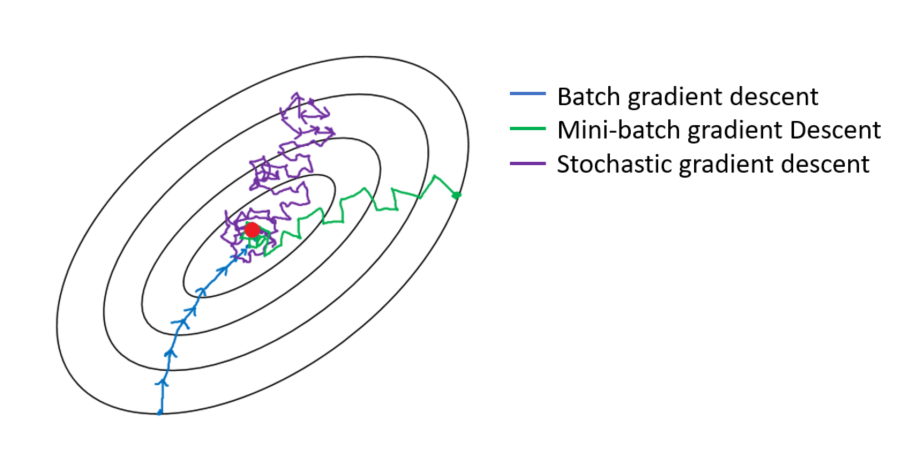
\includegraphics[width=\textwidth,height=\textheight,keepaspectratio]{minibatch_comparison}
    % \caption{\label{fig:label} }
  \end{figure}
\end{frame}


\begin{frame}
  \frametitle{Stochastic Subgradient Method}
  If we go back to the proof: We did not use smoothness. If we choose \textcolor{blue}{unbiased estimate of subgradient} $\E[g_k|x_k] \in \partial f(x_k)$ and iterate
  \begin{block}{}
    \begin{align}
      &\text{sample $i\in 1,\dots, n$ uniformly at random} \\
      &\text{let $g_k \in \partial f_i(x_k)$}\\
      &x_{k+1} = x_k - \alpha g_k.
    \end{align}
  \end{block}
  We can get the same $\mathcal{O}(\epsilon^{-2})$ complexity. Smoothness did provide any benefit (in terms of rate).
\end{frame}


\begin{frame}
  \frametitle{Projected SGD}

  \begin{itemize}
    \item Previous proof can be extended (trivially) to the constrained setting
    \item with same complexity $\mathcal{O}(\epsilon^{-2})$
    \item but (of course) additionaly
  \end{itemize}

\end{frame}

\section{High probability bounds}%
\label{sec:}

\begin{frame}
  \frametitle{High probability bounds}

  \begin{theorem}{Hoeffding's inequality}
    Let $X_i$ be independent random variables that satisfy
    \begin{itemize}
      \item $\E X_i = 0$
      \item $\Vert X_i \Vert \le M$.
    \end{itemize}
    Then,
    \begin{equation}
      \P\left[ X_1+ \dots + X_k \ge t\right] \le e^{-\frac{t^2}{2kM^2}}
    \end{equation}
  \end{theorem}

  Azuma-Hoeffding's generalization does not require independence, only $\E[X_k| X_{k-1}, \dots, 1]=0$.
\end{frame}


\begin{frame}
  \frametitle{Statement with high probability}
  \begin{theorem}
    Let $\delta>0$ and assumptions as before + iterates remain in bounded set with diameter $D$ (for example constraint set). Then,
    \begin{equation}
       f(\bar{x}_i) - f^* \le \frac{D B \delta}{\sqrt{k}}.
    \end{equation}
    with \textcolor{blue}{probability} less than $1-e^{-\delta^2/8}$.
  \end{theorem}
  $\Rightarrow$ choose $\delta$ large for bound in higher probability.
\end{frame}


\begin{frame}
  \begin{adjustwidth}{-1.5em}{-1.5em}
    \begin{minipage}{1.1\textwidth}
    \begin{proof}
      \begin{equation}
        \begin{aligned}
          \MoveEqLeft \Vert x_{k+1} - x^* \Vert^2 \\
          &\le \Vert x_k-x^* \Vert^2 + 2 \alpha \langle g_k, x^*-x_k \rangle + \alpha^2 \Vert g_k \Vert^2 \\
          &\le \Vert x_k-x^* \Vert^2 + 2 \alpha \langle \nabla f(x_k), x^*-x_k \rangle + \alpha^2 \Vert g_k \Vert^2  + \langle v_k, x^*-x_k \rangle\\
        \end{aligned}
      \end{equation}
      with $v_k = g_k -\nabla f(x_k)$.
      Continue as usual
      \begin{equation}
        f(\bar{x}_k) - f^* \le \frac{\Vert x_0-x^* \Vert^2}{2 \alpha k} + \alpha B^2 + \frac{1}{k} \sum_{i=1}^{k} X_i
      \end{equation}
      with
      \begin{equation}
        X_k := \langle v_k, x^*-x_k \rangle \le \Vert v_k \Vert \Vert x_k-x^* \Vert \le 2BD
      \end{equation}
      and $\E[X_k]=0$ fulfilling Hoeffding's assumptions. Use it with $t= DB \sqrt{k}\delta$.
    \end{proof}
    \end{minipage}
  \end{adjustwidth}
\end{frame}


\end{document}
